\documentclass[final]{article}

\usepackage[paperwidth=84.1cm,paperheight=118.9cm,margin=3cm]{geometry}
\usepackage{graphicx}
\usepackage{xcolor}
\usepackage[most]{tcolorbox}
\usepackage{tikz}
\usepackage{parskip}

\usepackage{amsmath, amssymb}
\usepackage{caption}
\usepackage{enumitem}

\pagestyle{empty}
\renewcommand{\familydefault}{\sfdefault}
\graphicspath{{LaTeX/images/}{Abschlussarbeit_2021/LaTeX/images/}}

\definecolor{uulmgray}{RGB}{70,70,70}
\definecolor{posterline}{RGB}{220,220,220}
\definecolor{posterfill}{RGB}{255,255,255}
\definecolor{posteraccent}{RGB}{0,104,125}
\definecolor{posteraccentlight}{RGB}{232,245,248}
\definecolor{postercallout}{RGB}{255,248,230}

\newcommand{\postertitle}{}
\newcommand{\posterauthor}{}
\newcommand{\posterinfo}{}

\captionsetup{font=small,labelfont=bf}
\setlist[itemize]{leftmargin=1.2em,itemsep=0.25em,topsep=0.25em}
\setlist[enumerate]{leftmargin=1.4em,itemsep=0.3em,topsep=0.3em}

\tcbset{
  posterblockstyle/.style={
    enhanced,
    colback=posterfill,
    colframe=posterline,
    coltitle=uulmgray,
    fonttitle=\huge\bfseries,
    fontupper=\Large,
    boxrule=1.5pt,
    arc=8mm,
    left=1.2cm,
    right=1.2cm,
    top=1cm,
    bottom=1cm,
    title filled=false,
    attach title to upper={\par\vspace{0.5cm}},
    borderline west={7pt}{0pt}{posteraccent},
    drop fuzzy shadow=black!10,
  },
  posteraccentblockstyle/.style={
    posterblockstyle,
    colback=posteraccentlight,
    colframe=posteraccent,
    top=1cm,
  },
  posterquestionstyle/.style={
    enhanced,
    colback=postercallout,
    colframe=posteraccent!45,
    boxrule=1pt,
    arc=5mm,
    left=0.8cm,
    right=0.8cm,
    top=0.6cm,
    bottom=0.6cm,
  },
  posterequationstyle/.style={
    enhanced,
    colback=white,
    colframe=posteraccent!25,
    boxrule=1pt,
    arc=5mm,
    left=0.6cm,
    right=0.6cm,
    top=0.25cm,
    bottom=0.25cm,
  }
}

\newcommand{\posterblock}[2]{%
  \begin{tcolorbox}[posterblockstyle,title={#1}]
    #2
  \end{tcolorbox}
  \vspace{1.3cm}
}
\newcommand{\posteraccentblock}[2]{%
  \begin{tcolorbox}[posteraccentblockstyle]
    \tikz[baseline=(label.base)] \node[
      fill=posteraccent,
      text=white,
      rounded corners=5pt,
      inner xsep=0.8cm,
      inner ysep=0.3cm,
      font=\huge\bfseries
    ] (label) {#1};
    \par\vspace{0.7cm}
    #2
  \end{tcolorbox}
  \vspace{1.3cm}
}
\newcommand{\posterequation}[1]{%
  \begin{tcolorbox}[posterequationstyle]
    #1
  \end{tcolorbox}
}
\newcommand{\posterquestion}[1]{%
  \begin{tcolorbox}[posterquestionstyle]
    \textbf{Question.} #1
  \end{tcolorbox}
}

\begin{document}
\begin{tikzpicture}[remember picture,overlay]
  \draw[posterline,line width=1.5pt]
    ([xshift=3cm,yshift=-8cm]current page.north west) --
    ([xshift=-3cm,yshift=-8cm]current page.north east);
\end{tikzpicture}

\begin{minipage}[t]{0.68\textwidth}
  {\Huge\bfseries\postertitle\par}
  \vspace{0.8cm}
  {\Large\posterauthor\par}
  \vspace{0.3cm}
  {\large\posterinfo\par}
\end{minipage}
\hfill
\begin{minipage}[t]{0.24\textwidth}
  \raggedleft
  
\includegraphics[width=0.85\linewidth]{logo_uulm_sw.png}
\end{minipage}

\vspace{3cm}

\begin{minipage}[t]{0.48\textwidth}
  \posteraccentblock{Why Select One Scale?}{
    Persistent homology records features across all filtration values. This is
    the right multiscale summary, but several downstream tasks still require
    one representative complex.

    \begin{itemize}
      \item Reconstruction and meshing need one complex with the right homotopy type.
      \item Topology-aware clustering depends on a neighborhood scale.
      \item Mapper and graph construction require local thresholds.
      \item Statistical tests on point processes often evaluate Betti numbers at selected scales.
    \end{itemize}

    The goal is therefore not to replace the persistence diagram, but to turn it
    into an operational scale choice.
  }

  \posterblock{Spectral Scale Selection}{
    Let $K_1,\dots,K_N$ be complexes from a filtration, for example
    $K_i=\mathrm{VR}_{\epsilon_i}(X)$, $\check{C}_{\epsilon_i}(X)$, or
    $\alpha_{\epsilon_i}(X)$. For a functional $f$ on simplicial complexes,
    define the scale interaction by

    \posterequation{
      \[
        \langle K_i,K_j\rangle_f
        = f(K_i)+f(K_j)-f(K_i\oplus K_j),
        \qquad
        \Sigma^{(N)}_{ij}=\langle K_i,K_j\rangle_f .
      \]
    }

    In the filtration case with the union operation this reduces to a min/meet
    matrix:

    \posterequation{
      \[
        \Sigma^{(N)}_{ij}=f(K_{\epsilon_{i\wedge j}}),
        \qquad i\wedge j=\min\{i,j\}.
      \]
    }

    The functional is chosen to combine topology and combinatorics:

    \posterequation{
      \[
        f(K)=f_{\mathrm{Top}}(K)\,f_{\mathrm{Comb}}(K)
      \]
      \[
        f_{\mathrm{Top}}(K)=
        \delta_{-1}+\sum_{j=0}^{d-1}\delta_j\beta_j^{\alpha_j}(K),
        \qquad
        f_{\mathrm{Comb}}(K)=
        \gamma_{-1}+\sum_{j=0}^{d}\gamma_j f_j^{\xi_j}(K).
      \]
    }

    The Perron vector ranks scales by their interaction with the entire
    filtration:
    \[
      \Sigma^{(N)}v^*=\lambda^*v^*,
      \qquad
      i_{\mathrm{crit}}\in\arg\max_{1\leq i\leq N}v_i^* .
    \]

    \posterquestion{
      Which scale is most strongly supported by all other scales, not only by
      its own value $f(K_i)$?
    }
  }

  \posterblock{PCA and Markov Chain View}{
    The scale similarity matrix plays the role of a covariance matrix on the
    space of scales. Its dominant eigenvector is analogous to the first
    principal component: it identifies the scale direction carrying the strongest
    cross-scale signal.

    \posterequation{
      \[
        P=\frac{1}{\lambda^*}D_{v^*}^{-1}\Sigma^{(N)}D_{v^*},
        \qquad
        \pi_i=\frac{(v_i^*)^2}{\|v^*\|_2^2}.
      \]
    }

    This is Doob's $h$-transform. It turns $\Sigma^{(N)}$ into a reversible
    Markov chain on the state space of scales. Scales with high stationary mass
    are globally supported by the filtration.

    \textbf{Non-monotone case.}
    The Perron ranking is the main selection rule. It is most informative when
    $i\mapsto f(K_{\epsilon_i})$ is not merely monotone, for instance when
    $\beta_0$ decreases while the edge count $f_1$ increases.

    \textbf{Monotone case.}
    If $f$ is monotone, the min matrix mainly reflects this monotonicity. Then
    the inverse matrix gives a birth-death chain with generator
    \[
      \mathcal{L}
      =\frac{1}{c_1}\mathrm{diag}(1,0,\dots,0)-(\Sigma^{(N)})^{-1},
      \qquad c_i=f(K_{\epsilon_i}).
    \]
    The critical scale is selected where the embedded chain has minimal
    stationary mass:
    \[
      i_{\mathrm{crit}}\in
      \arg\min_{1\leq i\leq N}\pi_i^{\mathrm{BD}}.
    \]
  }
\end{minipage}
\hfill
\begin{minipage}[t]{0.48\textwidth}
    \posterblock{The Mapper Algorithm}{
    Curabitur sed velit non urna congue vestibulum. Use this block for results,
    diagrams, images, equations, or other poster material.
  }

  \posterblock{Multiscale $\alpha$ Neighboring graph}{
    \begin{center}
        \begin{minipage}[t]{0.47\linewidth}
            \vspace{0pt}
            \centering
            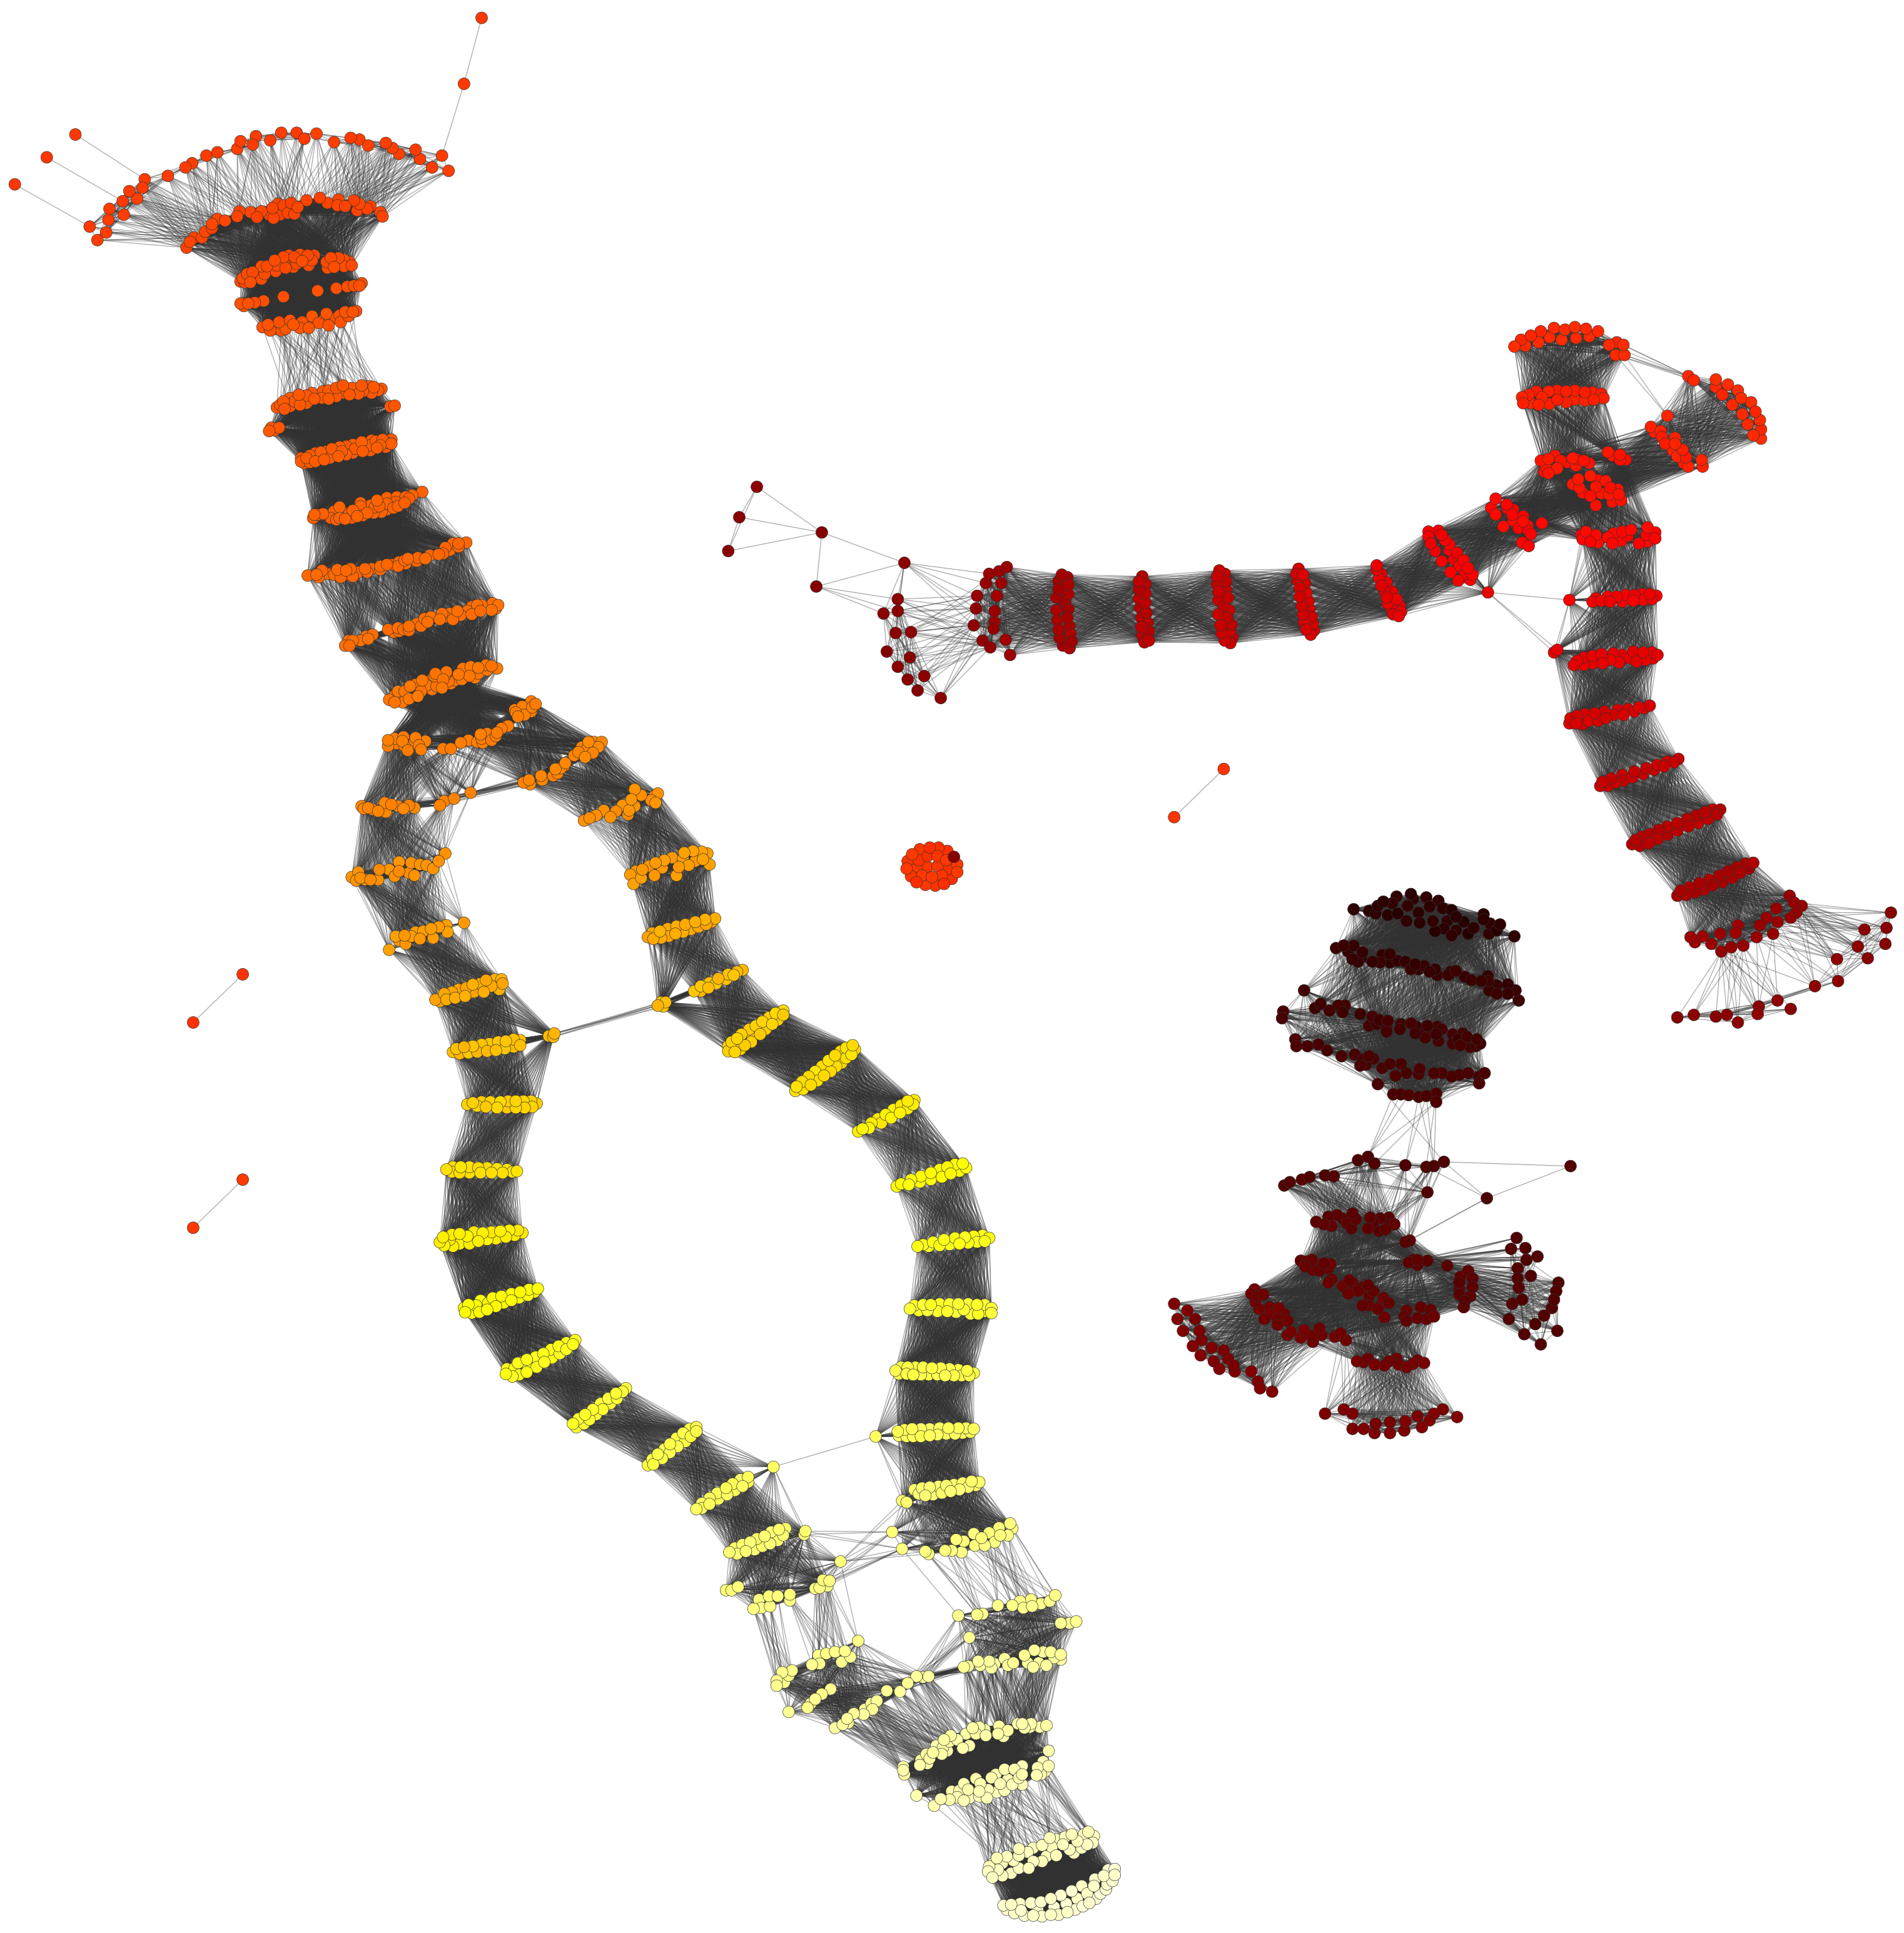
\includegraphics[width=\linewidth]{eight_fail.png}
            \captionof{figure}{First caption}
        \end{minipage}
        \hfill
        \begin{minipage}[t]{0.47\linewidth}
            \vspace{0pt}
            \centering
            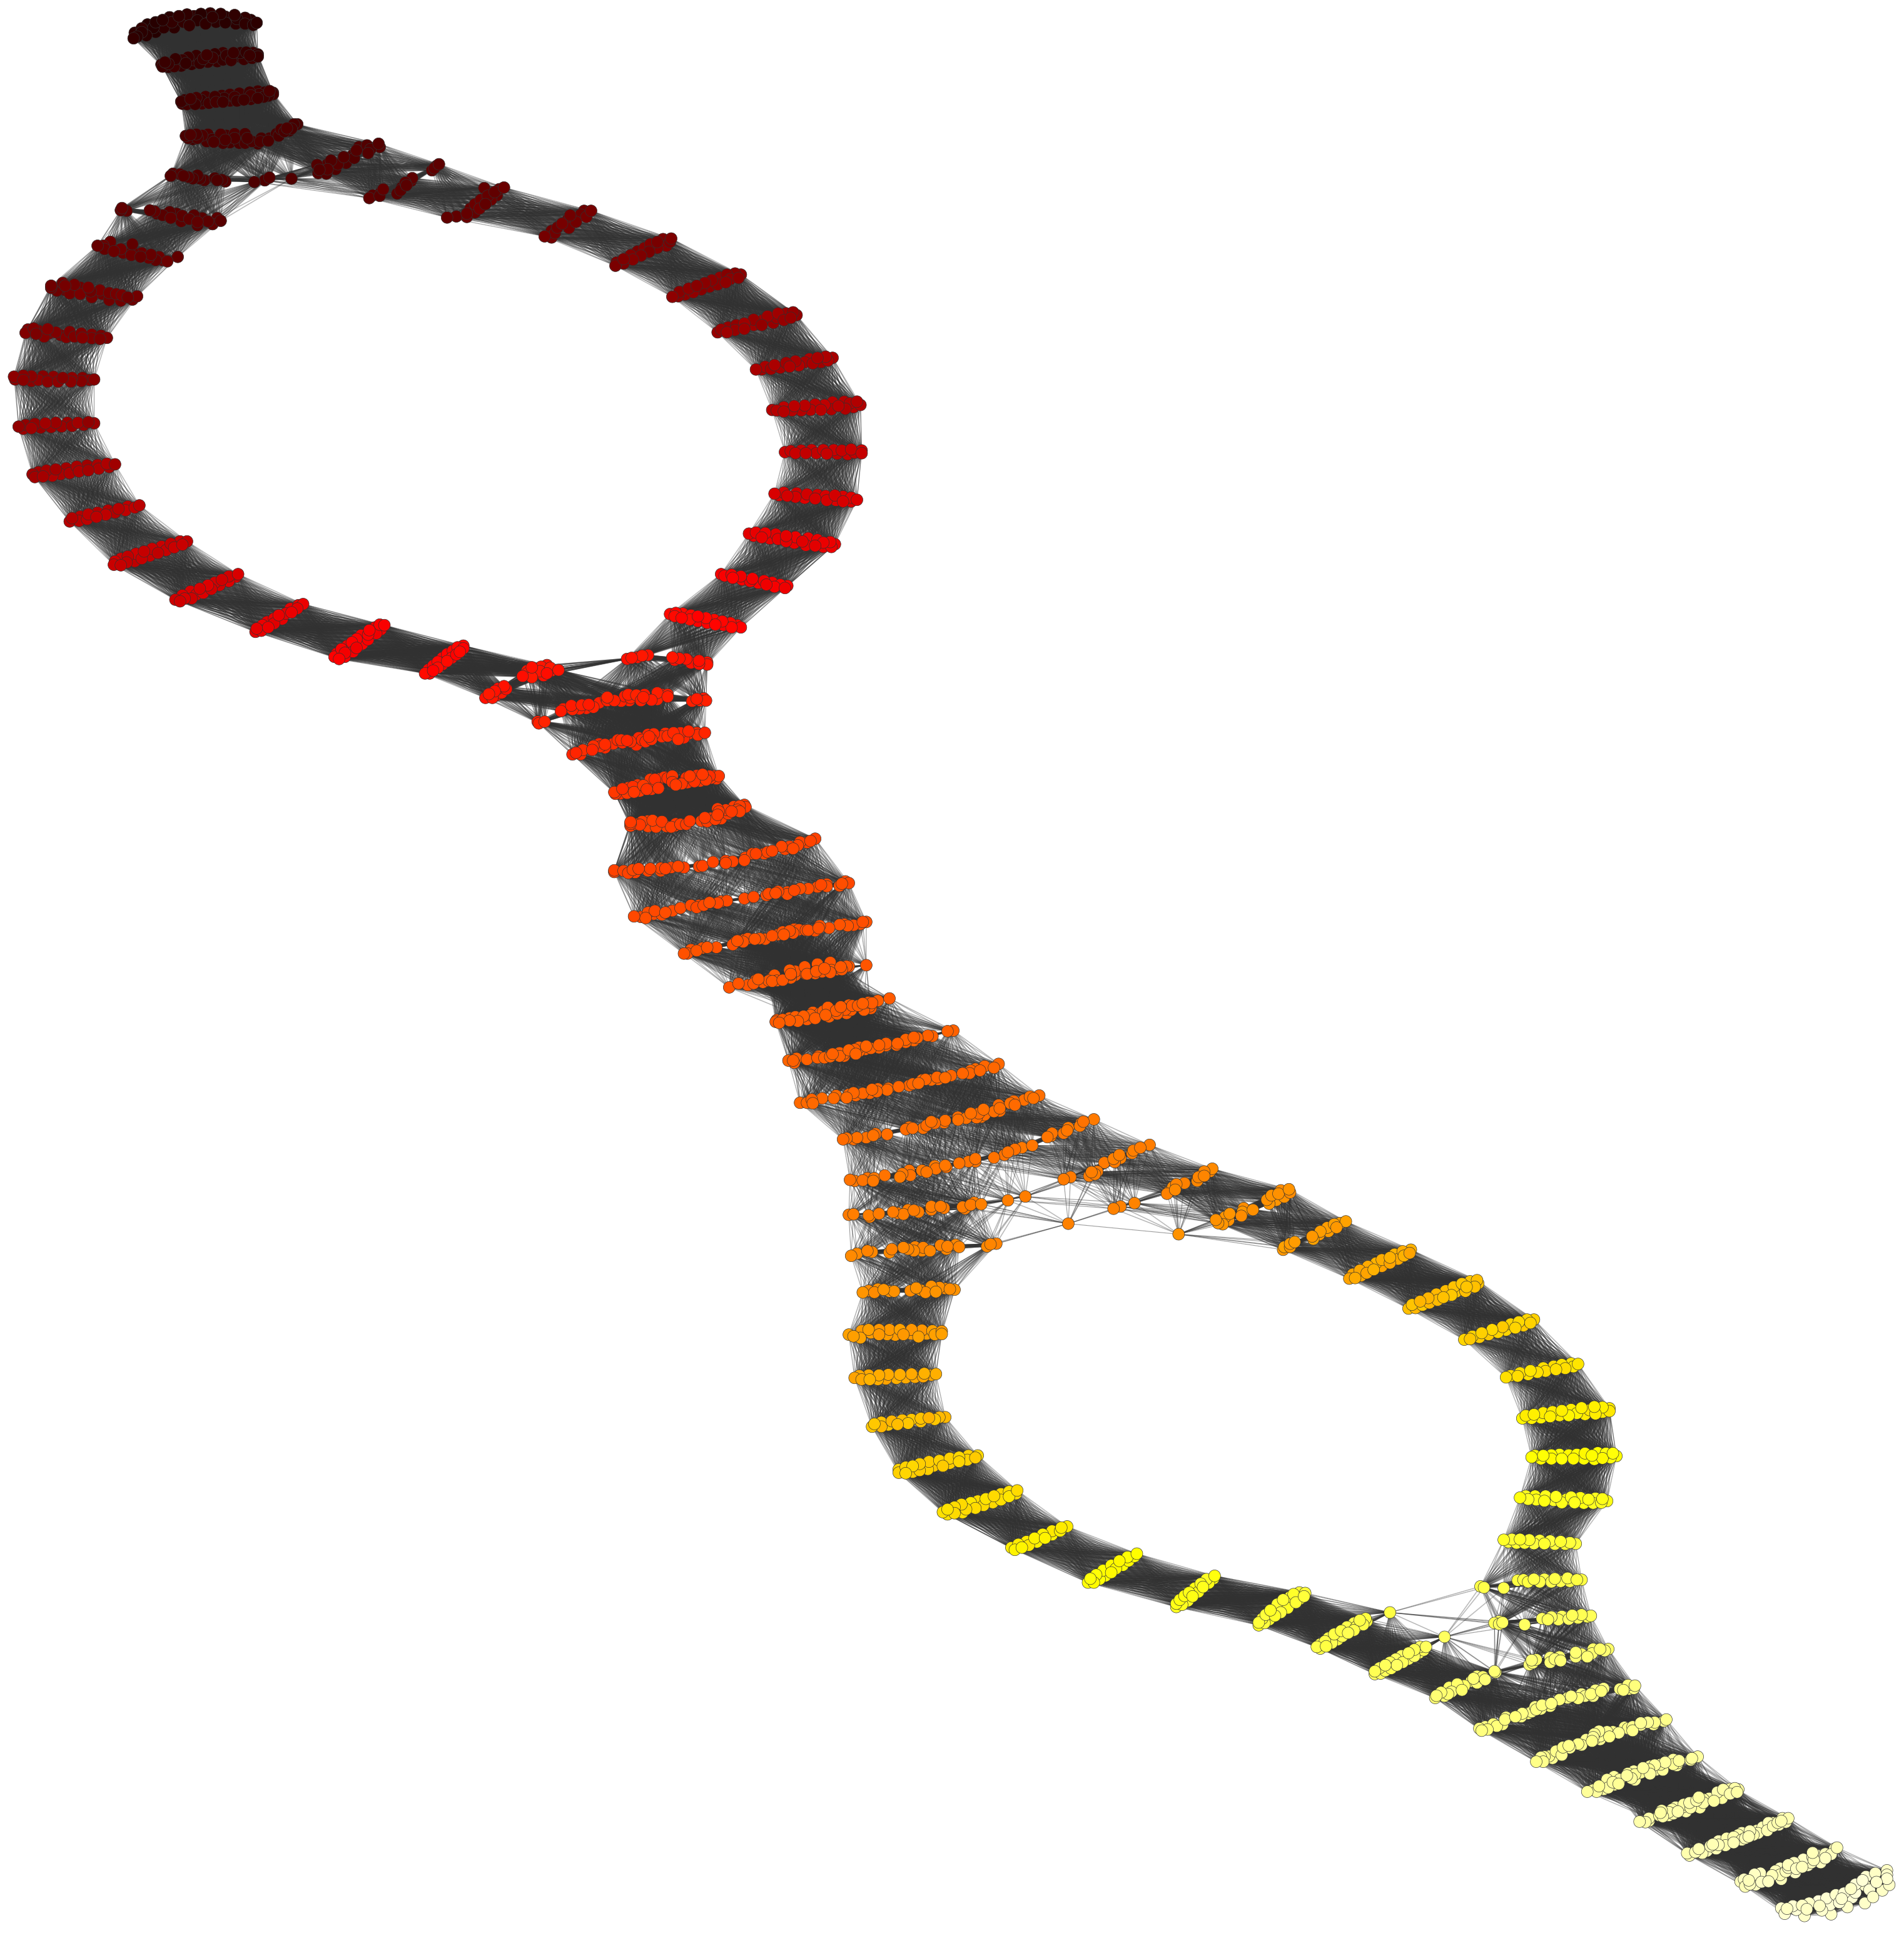
\includegraphics[width=\linewidth]{eight_proper.png}
            \captionof{figure}{Second caption}
        \end{minipage}
    \end{center}
}

  \posterblock{Case Study: Covid-19 Spread in the USA}{
    \begin{center}
        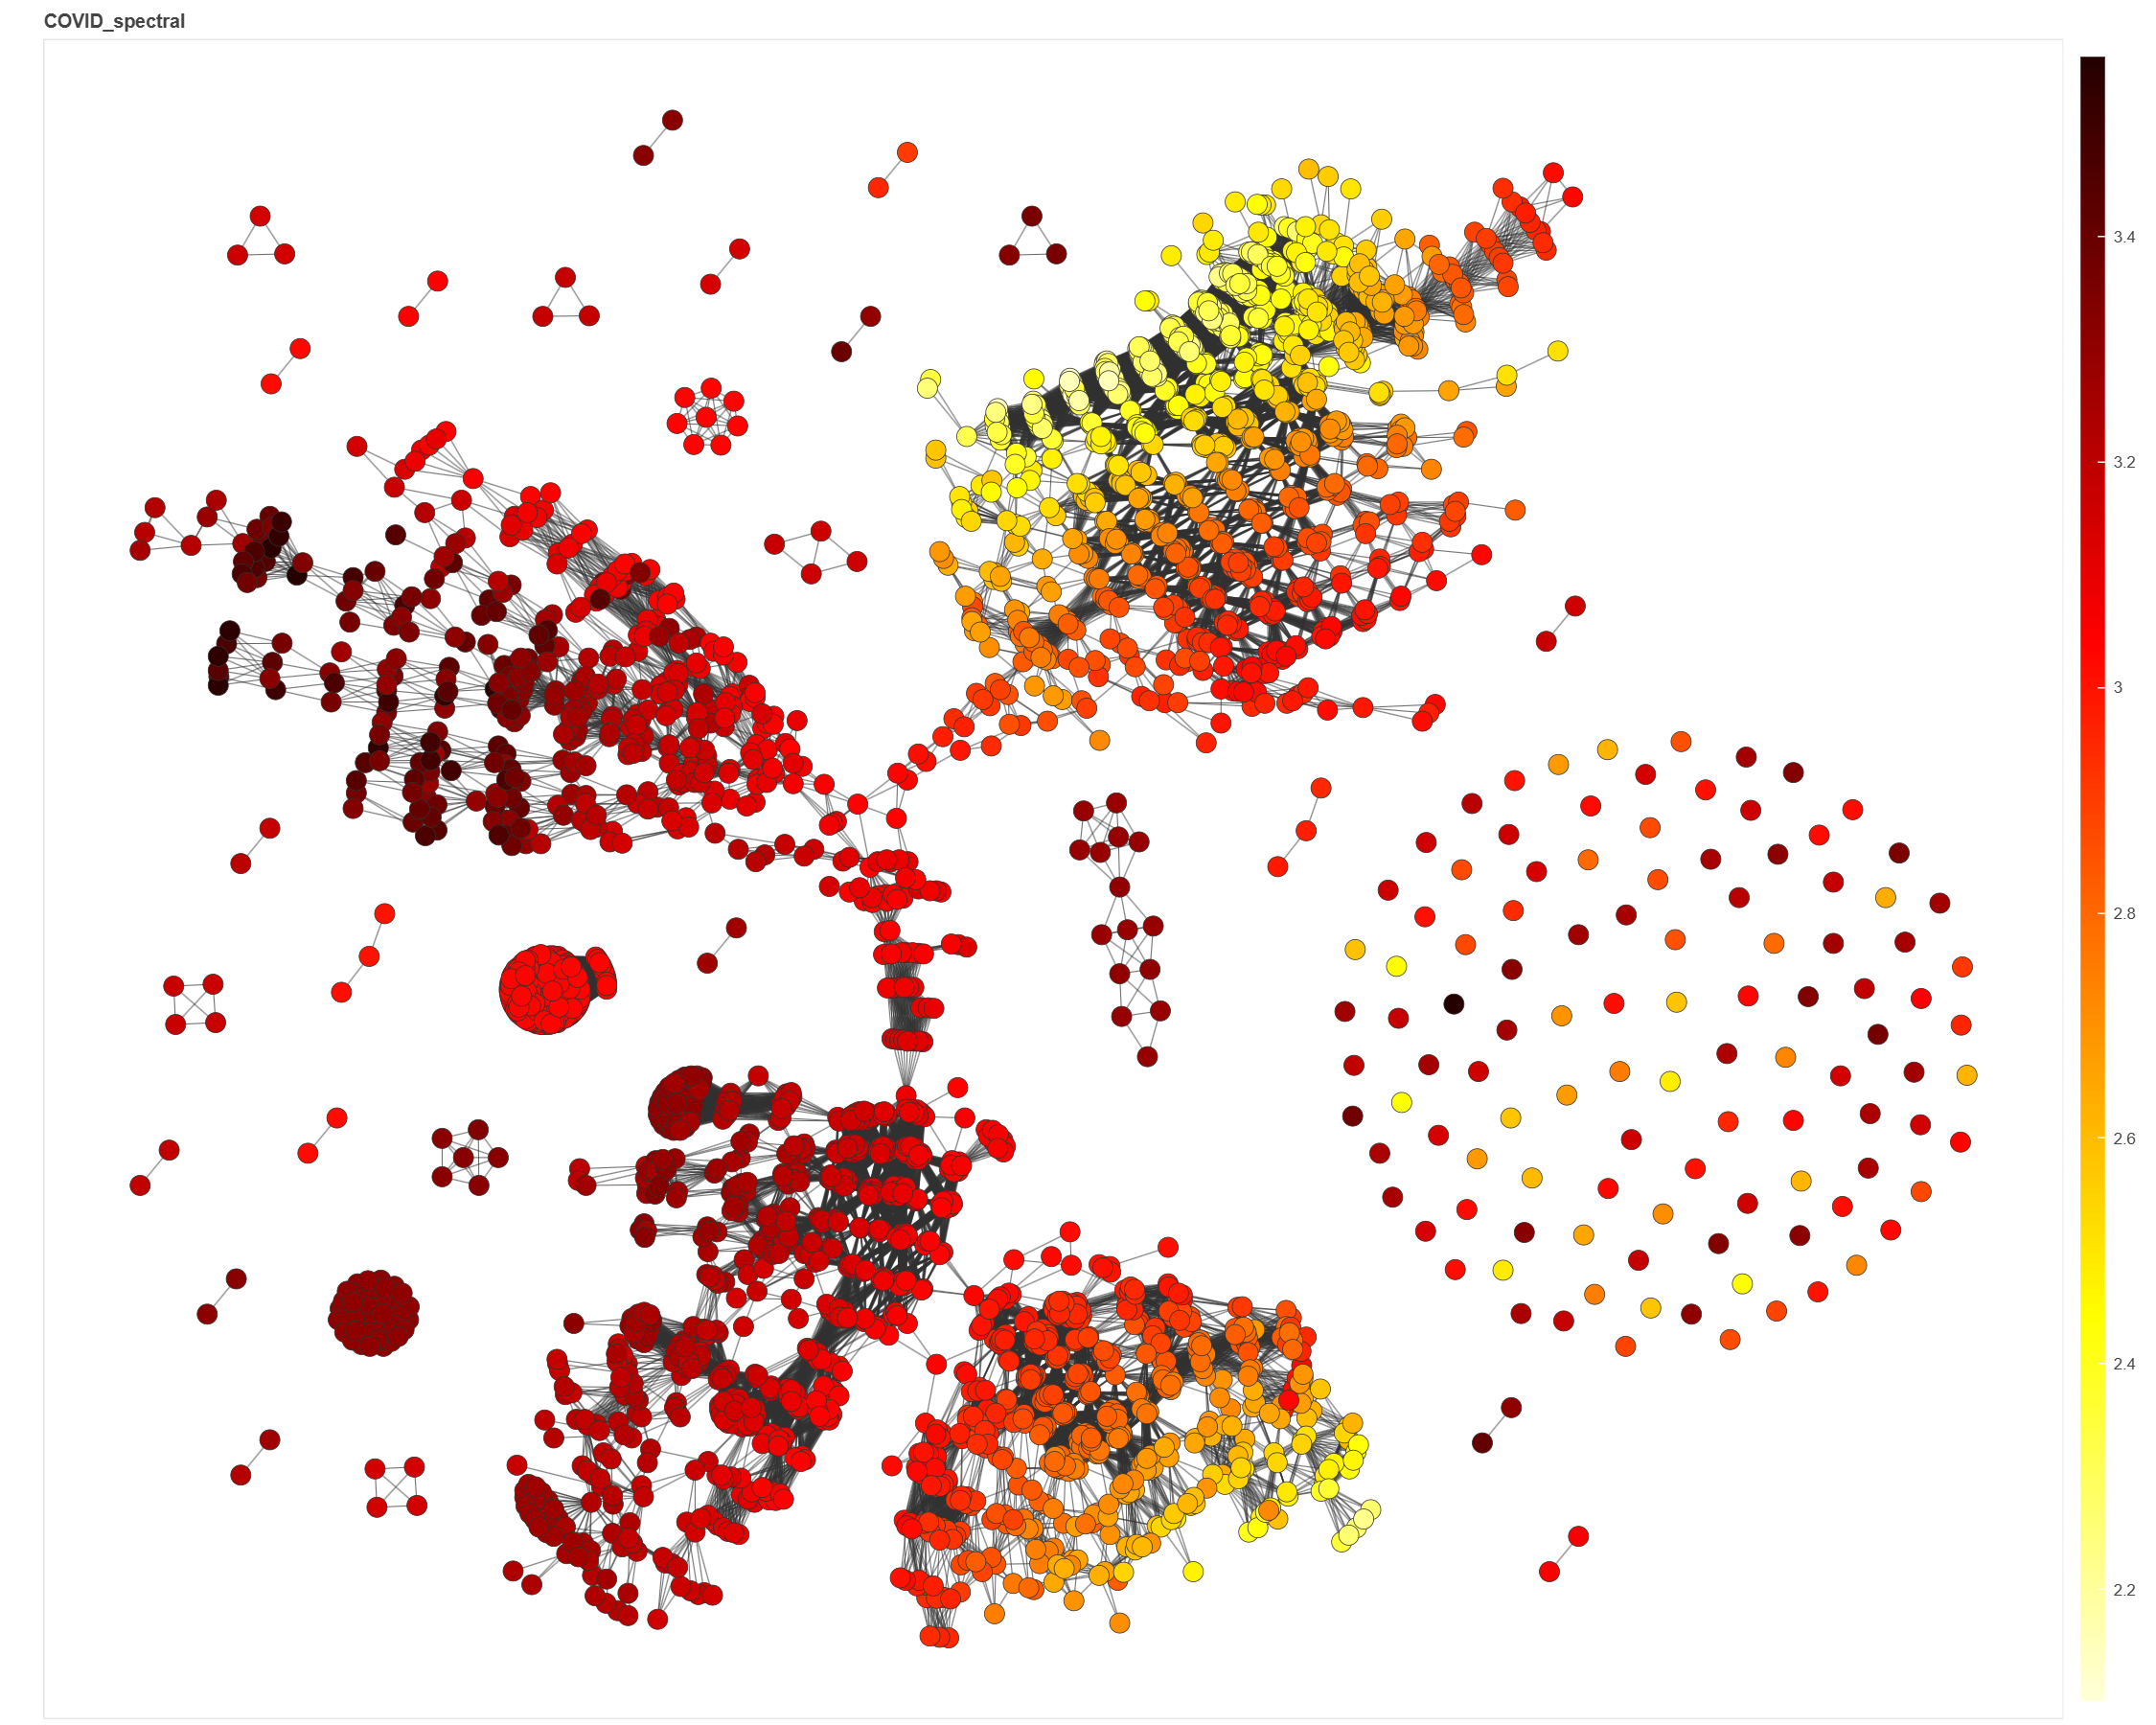
\includegraphics[width=0.8\linewidth]{COVID-projections_coloring.png}
        \captionof{figure}{Caption}
        \label{fig:placeholder}
    \end{center}
}
\end{minipage}

\end{document}
